\documentclass{article}
\usepackage[margin=.9in]{geometry}
\usepackage{xcolor}
\usepackage{amsmath}
\usepackage{amssymb}
\usepackage{float}
\usepackage{listings}
\usepackage{natbib}
\usepackage{booktabs}
\setlength{\parindent}{0pt}
\setlength{\parskip}{\baselineskip}
\definecolor{mycolor}{rgb}{0.1, 0.1, 0.5}
\title{\textcolor{mycolor}{\textbf{{\huge Development and Implementation of a Low-Cost Electrochemistry Lab Kit for Educational Outreach: Methodology}}}}
\author{Student: Christopher Hunt \\ Mentor: Dr. Kelsey Stoerzinger}
\date{}
\usepackage{graphicx} 
\usepackage{fancyhdr}

\begin{document}
\pagestyle{fancy}
\fancyhf{}
\rfoot{}
\lfoot{Christopher Hunt}
\lhead{Development and Implementation of a Low-Cost Electrochemistry Lab Kit for Educational Outreach: Methodology}
\rhead{\thepage}
\maketitle
\subsection*{Introduction}
This research undertakes an examination, construction, and testing of various Arduino-based potentiostat designs. After examining several designs, we focused our attention on the Meloni Design due to its detailed circuit layout and ease of replication. We further enhanced this design by incorporating a 10-bit digital-analog converter to achieve a higher resolution control signal. Due to the limitations of this DIY potentiostat, specific component choices and layout may require adjustments to accurately provide data for our use case. The design will be constructed to properly detect the current generated from a Ferricyanide/Ferrocyanide redox reaction during a cyclic voltammetry (CV) experiment, the common benchmark test for the articles examined in our literature review. The methodology section thus elaborates on the research design, data collection, data analysis processes, and the limitations encountered in the study.

\subsection*{Research Design}
A comparative analysis of Arduino-based designs was performed. Arduino microcontrollers are known for their affordability and ease of implementation. From our literature review, it was determined that the hardware design will reflect the design choices made in The Meloni Design. This was chosen based on its detailed schematic and commonality in the potentiostat designs literature. This design, however, may require adjustments to the control signal and several component values to be operable within our research's specific test case.

The Meloni Design is comprised of 7 stages (fig. 1).
\begin{enumerate}
    \item Software-generated Pulse Width Modulated (PWM) control signal
    \item Hardware filtering of control signal
    \item Control signal biasing
    \item Potentiostat control amplifier
    \item Current to voltage conversion
    \item Output signal buffer
    \item Output signal software processing
\end{enumerate}

\begin{figure}[H]
    \centering
    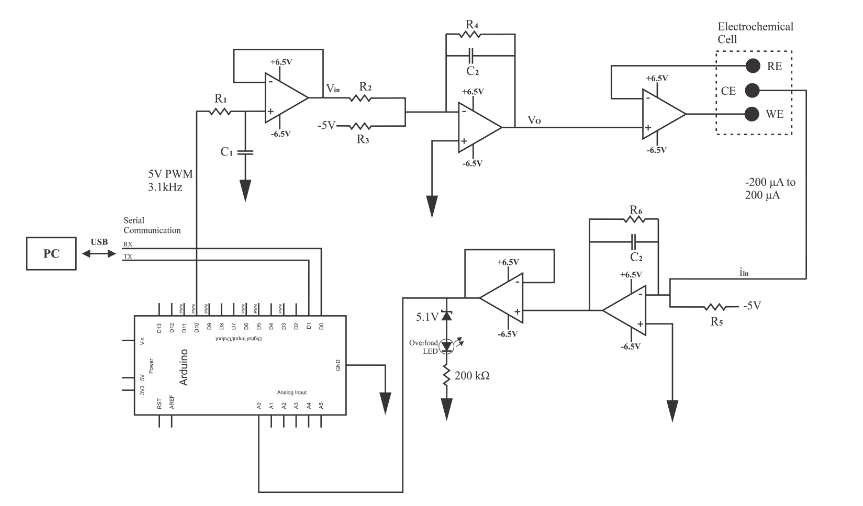
\includegraphics[width=.7\linewidth]{meloni_design.png}
    \caption{Meloni Design}
\end{figure}

The electrochemical reaction to be studied is a ferricyanide/ferrocyanide redox reaction. This reaction will first be conducted using a BioLogic VSP-300 potentiostat using the EC-Lab software. A CV will be produced using a potential window from 0 to 0.5 volts, with scan rates of 20, 50, and 100 mV/s. This benchmark testing will provide an expected current range of the redox reaction. 

There are three design components that are being adjusted from the Meloni Design. First, we chose to change how the control signal is generated. The Meloni Design uses a single PWM pin from the Arduino in combination with an RC filter and an op-amp in an integrator configuration to produce the control signal for the CV. For our design, we chose to use a 10-bit Digital-Analog Converter (DAC) using an R2R ladder. This offers two benefits: first, it offers greater resolution for the control signal - 10-bit precision instead of 8-bit with the PWM design. Second, the R2R ladder is a fundamental circuit design used in entry-level electrical engineering coursework, whereas the PWM design may be considered more advanced. Second, we chose to swap the connections between the working electrode (WE) and the counter electrode (CE). This design decision was made with consultation from a BioLogic representative who claimed that since we are concerned about the current through the working electrode, it is assumed that measuring the current directly through it is the optimal design solution. Third, we must alter the values of the current to voltage converter. We will use the benchmark testing current maximum and minimum values to calculate the appropriate resistor and capacitor values for this circuit.

The modifications to the original Meloni Design were made in line with theoretical circuit analysis techniques. The use of an R2R ladder and the need for future students to perform circuit analysis to attenuate component values offer a greater learning opportunity for students.

\subsection*{Data Collection and Analysis}
We are adopting a twofold data collection process. First, we will collect circuit output measurements to validate each stage of the design. Each circuit’s output is evaluated every millisecond, resulting in a dense dataset. Next, we will compare the output of our enhanced Meloni Design against the benchmark BioLogic VSP-300 potentiostat. We chose the BioLogic VSP-300 due to its established performance and widespread use in the scientific community.

The acquired data will be processed using Python, which allows for flexible and precise analysis. Cyclic voltammetry of the Ferro-ferricyanide reaction, common in literature, will be performed to test and compare the potentiostats.

\subsection*{Research Limitations}
Our research, while thorough, encounters certain limitations. The resolution of the cyclic voltammetry control signal and the analog input detector is 4.88 millivolts, which may not be sufficient for some highly sensitive applications. In addition, aligning the output current to a 0-5V scale presents a challenge as it's not entirely accurate. The signal conversion hardware assumes a maximum and minimum current, which could be variable. If the current is outside this range, the sensor either outputs 0 or 1023, meaning the measurements could be clipped or skewed.

\subsection*{Conclusion}
This research presents a comprehensive methodology to assess, improve, and compare Arduino-based potentiostat designs. While there are some limitations, the study leverages the strengths of existing designs, particularly the Meloni Design, and contributes valuable enhancements to this field. Further studies can build on these findings, optimizing and addressing the identified limitations.

\end{document}
